\documentclass{article}

\usepackage{fancyhdr}
\usepackage{extramarks}
\usepackage{amsmath}
\usepackage{amsthm}
\usepackage{amsfonts}
\usepackage{tikz}
\usepackage[plain]{algorithm}
\usepackage{algpseudocode}
\usepackage{graphicx}
\usepackage{gensymb}
\usepackage{hyperref}
\usepackage{enumitem}
\usepackage{listings}
\usepackage{siunitx}
\usepackage{matlab-prettifier}

\DeclareRobustCommand{\bbone}{\text{\usefont{U}{bbold}{m}{n}1}}

\DeclareMathOperator{\EX}{\mathbb{E}}% expected value

\graphicspath{{./images/}}

\usetikzlibrary{automata,positioning}

%
% Basic Document Settings
%

\topmargin=-0.45in
\evensidemargin=0in
\oddsidemargin=0in
\textwidth=6.5in
\textheight=9.0in
\headsep=0.25in

\linespread{1.1}

\pagestyle{fancy}
\lhead{\hmwkAuthorName}
\chead{\hmwkClassShort\ \hmwkTitle}
\rhead{\firstxmark}
\lfoot{\lastxmark}
\cfoot{\thepage}

\renewcommand\headrulewidth{0.4pt}
\renewcommand\footrulewidth{0.4pt}

\setlength\parindent{0pt}

%
% Create Problem Sections
%

\newcommand{\enterProblemHeader}[1]{
    \nobreak\extramarks{}{Problem {#1} continued on next page\ldots}\nobreak{}
    \nobreak\extramarks{{#1} (continued)}{{#1} continued on next page\ldots}\nobreak{}
}

\newcommand{\exitProblemHeader}[1]{
    \nobreak\extramarks{{#1} (continued)}{{#1} continued on next page\ldots}\nobreak{}
    % \stepcounter{#1}
    \nobreak\extramarks{{#1}}{}\nobreak{}
}

\setcounter{secnumdepth}{0}
\newcounter{partCounter}

\newcommand{\problemNumber}{0.0}

\newenvironment{homeworkProblem}[1][-1]{
    \renewcommand{\problemNumber}{{#1}}
    \section{\problemNumber}
    \setcounter{partCounter}{1}
    \enterProblemHeader{\problemNumber}
}{
    \exitProblemHeader{\problemNumber}
}

%
% Homework Details
%   - Title
%   - Class
%   - Author
%

\newcommand{\hmwkTitle}{Assignment \#4}
\newcommand{\hmwkClassShort}{RBE 595 (FAIR-AV)}
\newcommand{\hmwkClass}{RBE 595 --- FAIR-AV}
\newcommand{\hmwkAuthorName}{\textbf{Arjan Gupta}}

%
% Title Page
%

\title{
    \vspace{2in}
    \textmd{\textbf{\hmwkClass}}\\
    % \textmd{\textbf{\hmwkTitle}}\\
    \textmd{\textbf{Assignment \#4}}\\
    \vspace{3in}
}

\author{\hmwkAuthorName}
\date{}

\renewcommand{\part}[1]{\textbf{\large Part \Alph{partCounter}}\stepcounter{partCounter}\\}

%
% Various Helper Commands
%

% Useful for algorithms
\newcommand{\alg}[1]{\textsc{\bfseries \footnotesize #1}}

% For derivatives
\newcommand{\deriv}[2]{\frac{\mathrm{d}}{\mathrm{d}#2} \left(#1\right)}

% For compact derivatives
\newcommand{\derivcomp}[2]{\frac{\mathrm{d}#1}{\mathrm{d}#2}}

% For partial derivatives
\newcommand{\pderiv}[2]{\frac{\partial}{\partial #2} \left(#1\right)}

% For compact partial derivatives
\newcommand{\pderivcomp}[2]{\frac{\partial #1}{\partial #2}}

% Integral dx
\newcommand{\dx}{\mathrm{d}x}

% Alias for the Solution section header
\newcommand{\solution}{\textbf{\large Solution}}

% Probability commands: Expectation, Variance, Covariance, Bias
\newcommand{\E}{\mathrm{E}}
\newcommand{\Var}{\mathrm{Var}}
\newcommand{\Cov}{\mathrm{Cov}}
\newcommand{\Bias}{\mathrm{Bias}}

\begin{document}

\maketitle

\nobreak\extramarks{Problem 1}{}\nobreak{}

\pagebreak

\begin{homeworkProblem}[Problem 1]

    Download PythonRobotics to a folder in your local 
    computer and run the fast\_slam2.py in 
    /PythonRobotics/SLAM/FastSLAM2.
    Capture a screen of the SLAM figure and the terminal you used to run the Python code.
    Upload the picture as the evidence of successfully running fast\_slam2.py.

    \section{Solution}

    After cloning the repository via git and running the recommended set up command which is as
    follows:

    \begin{lstlisting}[style=Matlab-editor]
        conda env create -f requirements/environment.yml
    \end{lstlisting}

    I created the conda environment and activated it. I then tried to run the \texttt{fast\_slam2.py}
    file in the \texttt{PythonRobotics/SLAM/FastSLAM2} directory. However, I ran into the error
    of the utils directory not being found. I then edited the \texttt{fast\_slam2.py} file to
    append the path of the parent's parent directory to the \texttt{sys.path} variable. This
    eliminated the error. After this I was able to successfully run the \texttt{fast\_slam2.py}
    file. The output of the terminal for these steps is shown in Figure \ref{fig:terminal}. 
    The output of the git diff command is shown in Figure \ref{fig:gitdiff} (this shows the lines I
    added to the \texttt{fast\_slam2.py} file). The output of the
    SLAM figure is shown in three different time points in the Figures \ref{fig:slam1}, \ref{fig:slam2},
    and \ref{fig:slam3}.

    \begin{figure}[H]
        \centering
        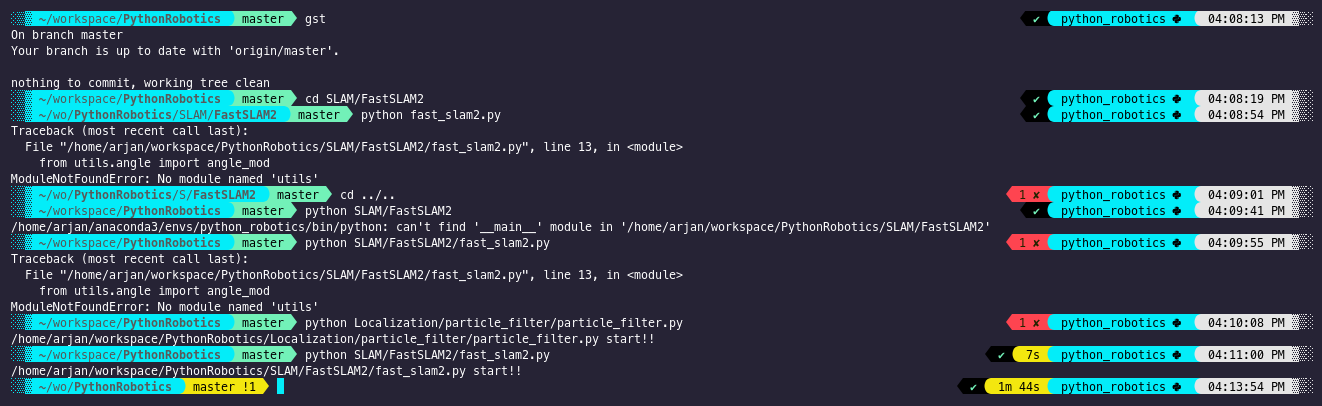
\includegraphics[width=\textwidth]{terminal_output.png}
        \caption{Output of the terminal steps to successfully run the \texttt{fast\_slam2.py} file.}
        \label{fig:terminal}
    \end{figure}

    \begin{figure}[H]
        \centering
        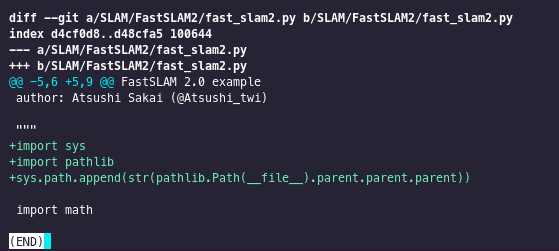
\includegraphics[width=\textwidth]{git-diff-output.png}
        \caption{Output of the git diff command to show the lines I added to the \texttt{fast\_slam2.py} file.}
        \label{fig:gitdiff}
    \end{figure}

    \begin{figure}[H]
        \centering
        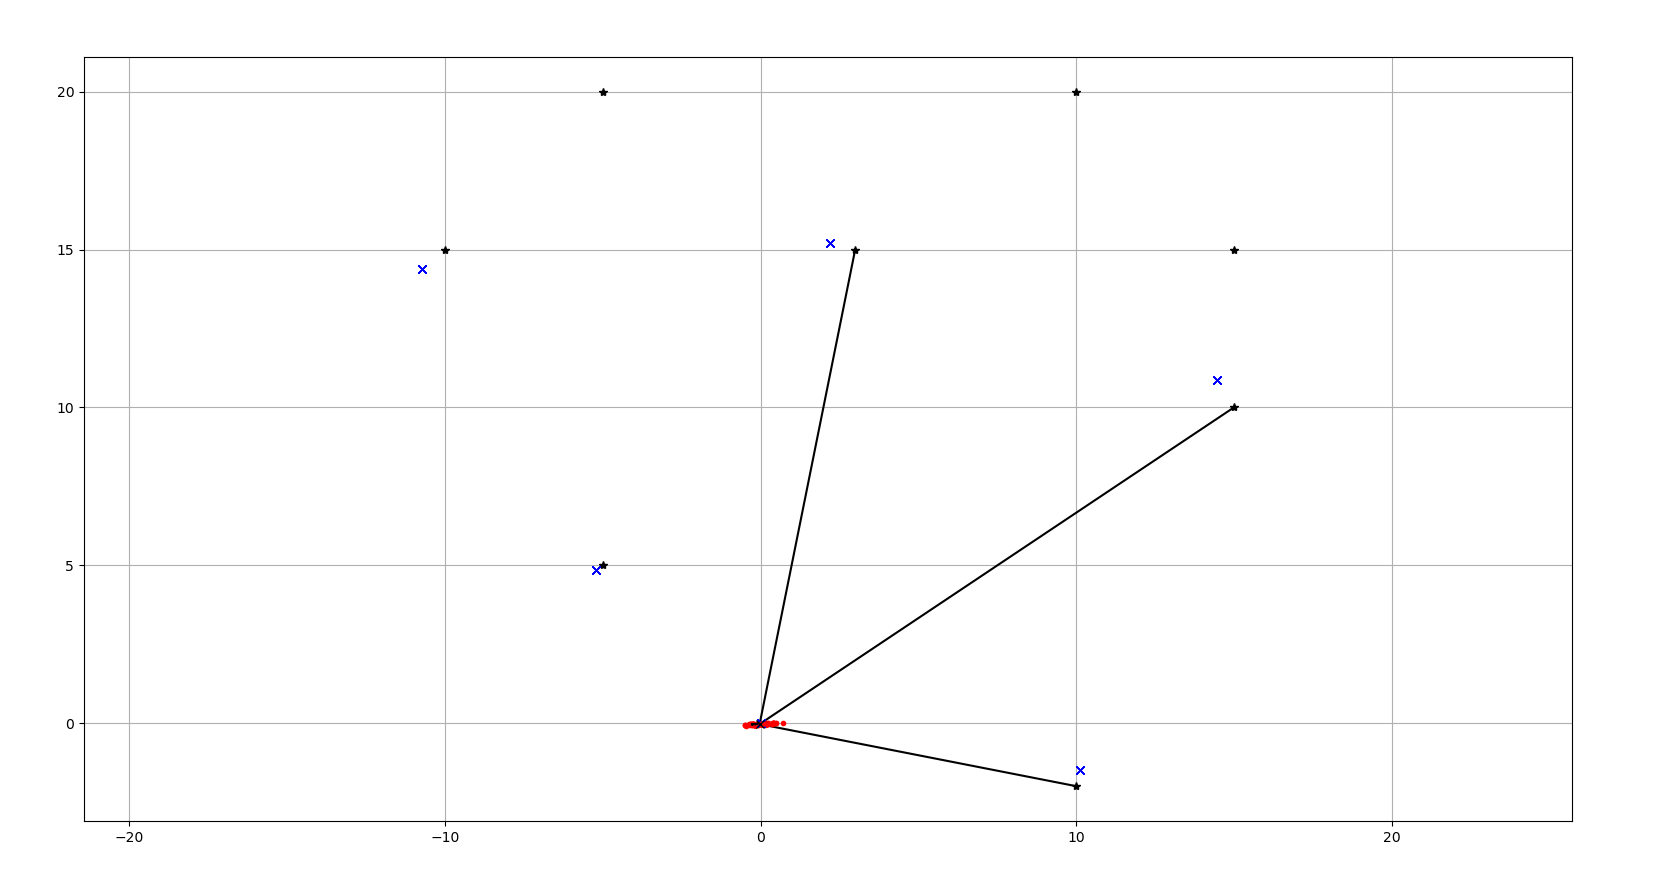
\includegraphics[width=\textwidth]{slam_capture1.png}
        \caption{Output of the SLAM figure at a few seconds into the run.}
        \label{fig:slam1}
    \end{figure}

    \begin{figure}[H]
        \centering
        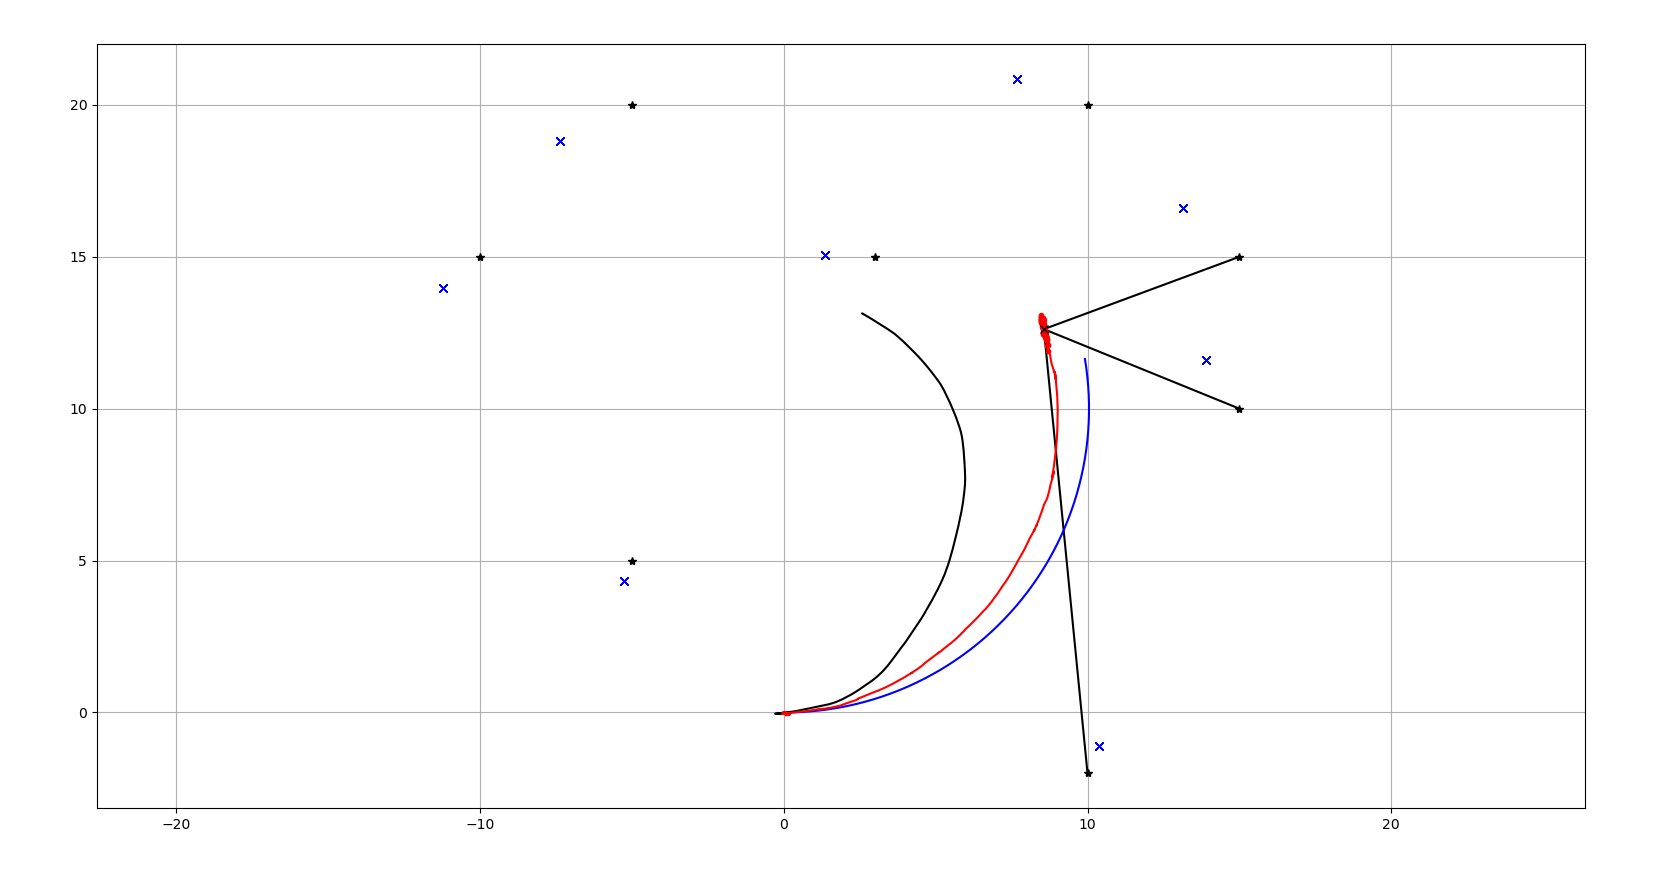
\includegraphics[width=\textwidth]{slam_capture2.png}
        \caption{Output of the SLAM figure about 30 seconds into the run.}
        \label{fig:slam2}
    \end{figure}

    \begin{figure}[H]
        \centering
        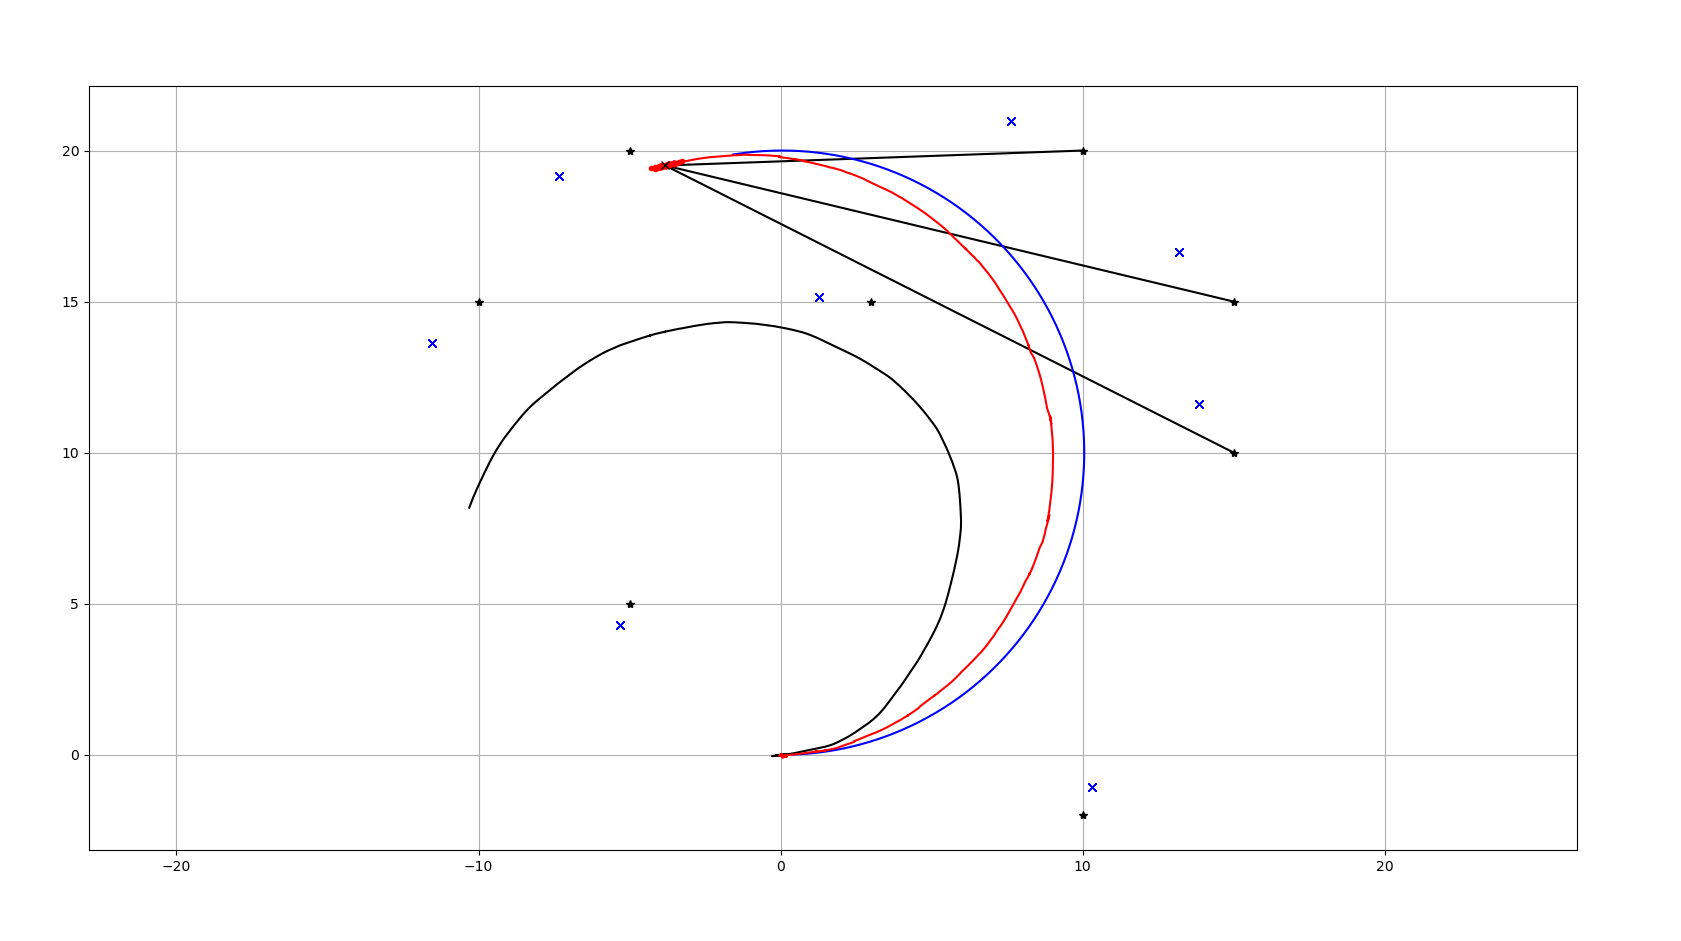
\includegraphics[width=\textwidth]{slam_capture3.png}
        \caption{Output of the SLAM figure after over a minute of the runtime.}
        \label{fig:slam3}
    \end{figure}

\end{homeworkProblem}

\end{document}